\documentclass[aspectratio=169,10pt]{beamer}
\usepackage[T1]{fontenc}
\usepackage[utf8]{inputenc}
\usepackage{helvet}
\usepackage{amsmath,booktabs,tabularx,array,ragged2e,colortbl}
\usepackage{tikz}
\usetikzlibrary{arrows.meta,positioning,calc}
\usepackage{fancyvrb}
\renewcommand{\familydefault}{\sfdefault}
\usefonttheme{professionalfonts}
\definecolor{Blue}{HTML}{2B5783}
\definecolor{MidBlue}{HTML}{5C86B1}
\definecolor{Ink}{HTML}{202D3A}
\definecolor{Muted}{HTML}{596774}
\definecolor{Pale}{HTML}{EDF3F7}
\definecolor{Line}{HTML}{BDCEDD}
\definecolor{Green}{HTML}{277C63}
\definecolor{Red}{HTML}{AF493F}
\definecolor{Teal}{HTML}{167C80}
\definecolor{Gold}{HTML}{BE8529}
\setbeamercolor{normal text}{fg=Ink,bg=white}
\setbeamercolor{structure}{fg=Blue}
\setbeamercolor{frametitle}{fg=Ink}
\setbeamercolor{block title}{fg=Blue,bg=Pale}
\setbeamercolor{block body}{fg=Ink,bg=Pale}
\setbeamercolor{code}{fg=Ink,bg=Pale}
\setbeamerfont{frametitle}{size=\fontsize{17}{20},series=\bfseries}
\setbeamerfont{block title}{size=\normalsize,series=\bfseries}
\setbeamertemplate{navigation symbols}{}
\setbeamertemplate{headline}{}
\setbeamersize{text margin left=.68cm,text margin right=.68cm}
\setbeamertemplate{frametitle}{\vspace{.16cm}\insertframetitle\par\vspace{.05cm}}
\setbeamertemplate{footline}{\hfill{\color{Blue}\fontsize{6.5}{7}\selectfont\insertframenumber}\hspace{.55cm}\vspace{.22cm}}
\setbeamertemplate{itemize item}{\color{Blue}\small\textbullet}
\setbeamertemplate{itemize subitem}{\color{Blue}\tiny\textbullet}
\setlength{\parskip}{.09cm}
\setlength{\tabcolsep}{5pt}
\renewcommand{\arraystretch}{1.3}
\newcolumntype{Y}{>{\RaggedRight\arraybackslash}X}
\newcolumntype{L}[1]{>{\RaggedRight\arraybackslash}p{#1}}
\newcommand{\hc}[1]{\textcolor{white}{\textbf{#1}}}
\newcommand{\subtitleline}[1]{{\color{Blue}\fontsize{8}{10}\selectfont #1\par}\vspace{.16cm}}
\newcommand{\takeaway}[1]{\par\vspace{.16cm}{\color{Blue}\bfseries #1\par}}
\newcommand{\source}[1]{\vfill{\color{Muted}\fontsize{5.8}{7.2}\selectfont #1\par}}
\newcommand{\smallbody}{\fontsize{9}{11}\selectfont}
\newcommand{\nei}{\textcolor{Blue}{\textbf{NOT ENOUGH INFO}}}
\newcommand{\supp}{\textcolor{Green}{\textbf{SUPPORTS}}}
\newcommand{\refu}{\textcolor{Red}{\textbf{REFUTES}}}
\tikzset{box/.style={draw=Line,fill=Pale,rounded corners=1pt,align=center,inner sep=7pt,font=\small},
 flow/.style={-{Stealth[length=2mm]},thick,draw=MidBlue}}
\hypersetup{pdftitle={Adversarial Fact Verification: Prompting and Fine-Tuning},pdfauthor={Team B},pdfsubject={Course project report, November 2026}}
\setbeameroption{hide notes}

\begin{document}

% 01 -- 5 seconds
\begin{frame}[plain]
\vspace{1.25cm}
\begin{center}
{\color{Blue}\fontsize{26}{30}\selectfont\bfseries Adversarial Fact Verification\par}
\vspace{.30cm}
{\color{MidBlue}\fontsize{14}{18}\selectfont Prompting and Fine-Tuning\par}
\vspace{.13cm}
{\color{MidBlue}\fontsize{11}{14}\selectfont Evidence-based classification of English person and event texts\par}
\vspace{.85cm}
{\fontsize{13}{16}\selectfont Team B\par}
\vspace{.18cm}
Course Project Report\par
\vspace{.12cm}
{\small November 2026}
\end{center}
\note{We study whether language models respect the boundaries of evidence in adversarial fact verification.}
\end{frame}

% 02 -- 20 seconds
\begin{frame}[t]{What Does the Evidence Establish?}
\subtitleline{Evidence + Claim $\longrightarrow$ Model $\longrightarrow$ SUPPORTS / REFUTES / NOT ENOUGH INFO}
{\small\supp: entailed\hfill\refu: contradicted\hfill\nei: neither}
\vspace{.17cm}
\begin{beamercolorbox}[sep=.15cm,wd=\textwidth]{code}
\small\textbf{Claim:} Akira Toriyama secretly donated five million yen to a local orphanage in Fukuoka.
\end{beamercolorbox}
\vspace{.16cm}
\begin{columns}[T,onlytextwidth]
\begin{column}{.48\textwidth}
{\color{Blue}\textbf{Evidence excerpt A}}\par
\smallbody His longtime editor at Shueisha \textbf{dismissed as baseless} the reports that Akira Toriyama had secretly donated five million yen to a local orphanage in Fukuoka.
\vspace{.12cm}\par
\textbf{Gold label:} \nei
\end{column}
\begin{column}{.48\textwidth}
{\color{Blue}\textbf{Evidence excerpt B}}\par
\smallbody Reports that Akira Toriyama had secretly donated five million yen to a local orphanage in Fukuoka were later \textbf{shown to be false}.
\vspace{.12cm}\par
\textbf{Gold label:} \refu
\end{column}
\end{columns}
\takeaway{Lack of support is not evidence of falsity.}
\source{Benchmark text; not a real-world factual claim. Verbatim excerpts from two development items in the same scenario group.\\Source: V16 revision 2 holdout, IDs \texttt{e\_b30e3a12162be36f} and \texttt{e\_072e61b1f738c059}.}
\note{Both items have the same claim. Dismissing a report as baseless states a source's position. Showing the report to be false establishes a contradiction. We classify the relation between the supplied evidence and claim, without using outside knowledge.}
\end{frame}

% 03 -- 15 seconds
\begin{frame}[t]{Basic Skills and Adversarial Challenges}
\subtitleline{Team A supplies the benchmark; Team B evaluates and improves the model.}
\vspace{.3cm}
\begin{tabularx}{\textwidth}{L{2.0cm}L{1.6cm}YY}
\rowcolor{Blue}\hc{Dataset}&\hc{Original size}&\hc{Content}&\hc{Purpose}\\
\rowcolor{Pale}\textbf{Basic}&900 items&Numbers, dates, locations, plans and facts&Check for loss of basic ability\\
\textbf{Challenge}&885 items&Seven adversarial reasoning mechanisms&Detect unsupported inferences\\
\end{tabularx}
\vspace{.7cm}
\begin{center}
{\color{Blue}\large Improve challenge performance\quad$\longleftrightarrow$\quad Preserve basic accuracy}
\end{center}
\takeaway{Evaluate the two datasets separately.}
\source{Source: benchmark\_1011 dataset documentation. These are original dataset sizes. The unified development comparison later uses 120 basic and 141 challenge items.}
\note{We track basic and challenge performance separately. The goal is to improve difficult evidence boundaries while preserving ordinary classification ability. The original benchmark sizes differ from the development comparison denominators used later.}
\end{frame}

% 04 -- 20 seconds
\begin{frame}[t]{Seven Traps in Evidence-Based Reasoning}
\begin{columns}[T,onlytextwidth]
\begin{column}{.53\textwidth}
\fontsize{8.0}{10}\selectfont
\begin{tabularx}{\linewidth}{L{1.82cm}Y}
\rowcolor{Blue}\hc{Mechanism}&\hc{Key distinction}\\
\rowcolor{Pale}DENIAL&A denial is not a disproof.\\
LOOKALIKE&Facts do not transfer between people.\\
\rowcolor{Pale}UNIQUE&One person's success does not exclude another's.\\
PRESUP&Earlier does not always mean an earlier calendar year.\\
\rowcolor{Pale}TEMPSCOPE&A first term does not cover all terms.\\
SETCLOSE&A complete subset is not the complete set.\\
\rowcolor{Pale}AMBIGREF&A pronoun about someone else does not refute the subject's claim.\\
\end{tabularx}
\end{column}
\begin{column}{.43\textwidth}
\smallbody
{\color{Blue}\textbf{UNIQUE: a benchmark item}}\par
\textbf{Evidence excerpt}\par
In 2024, Olivia Edgar-Jones won a regional theater award for best supporting actress.
\vspace{.09cm}\par
\textbf{Claim}\par
Daisy Edgar-Jones won a regional theater award for best supporting actress in 2024.
\vspace{.09cm}\par
\textbf{Gold label:} \nei
\vspace{.13cm}\par
{\color{Red}\textbf{Unsupported assumption:} only one person can win.}
\end{column}
\end{columns}
\takeaway{Identity, exclusivity, time and scope must come from the evidence.}
\source{Benchmark text; not a real-world factual claim. Source: development item \texttt{e\_51c3569118fd293c}, UNIQUE / other\_indef\,|\,indef. The assumption shown is an explanatory diagnosis, not an evidence quote or model transcript.}
\note{The seven mechanisms probe boundaries such as source stance, identity and scope. In this actual example, Olivia winning does not establish that Daisy failed to win. An unjustified exclusivity assumption turns missing information into a false contradiction.}
\end{frame}

% 05 -- 15 seconds
\begin{frame}[t,fragile]{Route 1: Direct Classification}
\subtitleline{The original A0 prompt provides the reference point.}
\begin{columns}[T,onlytextwidth]
\begin{column}{.43\textwidth}
\begin{center}
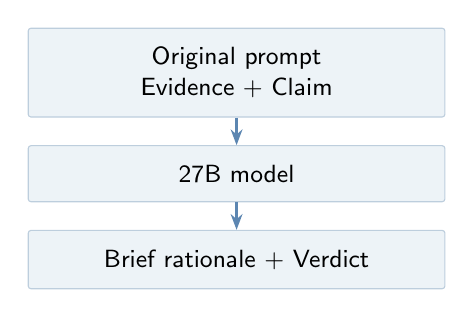
\begin{tikzpicture}[node distance=.35cm]
\node[box,text width=4.8cm] (a) {Original prompt\\Evidence + Claim};
\node[box,text width=4.8cm,below=of a] (b) {27B model};
\node[box,text width=4.8cm,below=of b] (c) {Brief rationale + Verdict};
\draw[flow] (a)--(b);\draw[flow] (b)--(c);
\end{tikzpicture}
\end{center}
\small One model call\par No weight updates
\end{column}
\begin{column}{.53\textwidth}
{\color{Blue}\textbf{Prompt excerpts}}\par
\begin{beamercolorbox}[sep=.18cm,wd=\linewidth]{code}
\begin{Verbatim}[fontsize=\scriptsize]
Judge the claim ONLY against the evidence
below; do not use outside knowledge.

EVIDENCE:
{evidence}

CLAIM: {claim}

Verdict: <SUPPORTS | REFUTES |
         NOT ENOUGH INFO>
\end{Verbatim}
\end{beamercolorbox}
\end{column}
\end{columns}
\takeaway{The baseline already defines all three logical relations.}
\source{Source: prompts/v1/A0\_user.txt. Excerpts omit surrounding instructions; line breaks are adjusted for display. V17 uses a brief justification followed by the final Verdict line.}
\note{The baseline already specifies entailment, contradiction and insufficient information. It asks the same model for a brief rationale and a final verdict. Our later methods address failures to apply those instructions consistently.}
\end{frame}

% 06 -- 20 seconds
\begin{frame}[t]{Route 2: Natural Language Inference}
\subtitleline{Reframe evidence verification as a premise--hypothesis relation.}
\vspace{.23cm}
\begin{columns}[T,onlytextwidth]
\begin{column}{.44\textwidth}
{\color{Blue}\large\textbf{Evidence = Premise}}\par
\vspace{.25cm}
{\color{Blue}\large\textbf{Claim = Hypothesis}}\par
\vspace{.4cm}
Does the premise entail the hypothesis or its negation?
\end{column}
\begin{column}{.51\textwidth}
\begin{tabularx}{\linewidth}{YY}
\rowcolor{Blue}\hc{NLI relation}&\hc{Verdict}\\
\rowcolor{Pale}Entailment&\supp\\
Contradiction&\refu\\
\rowcolor{Pale}Neutral&\nei\\
\end{tabularx}
\end{column}
\end{columns}
\vspace{.45cm}
\takeaway{Available evidence need not describe every fact about the world.}
\small One model call. No weight updates. Same rationale-and-verdict output.
\source{Source: V17 frozen prompts, NLI. Conceptual label mapping; the actual output uses Verdict, not an early JSON protocol.}
\note{NLI makes the premise--hypothesis relation explicit. In the award example, the evidence supports neither Daisy winning nor Daisy not winning, so the relation is neutral. We compare the full task framing rather than claiming that logical definitions are unique to this route.}
\end{frame}

% 07 -- 25 seconds
\begin{frame}[t]{Route 3: PJ Rule-Based Prompting}
\subtitleline{A shared prompt checks the assumptions behind a proposed contradiction.}
\begin{columns}[T,onlytextwidth]
\begin{column}{.45\textwidth}
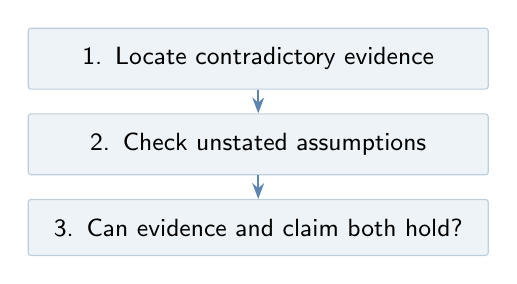
\begin{tikzpicture}[node distance=.30cm]
\node[box,text width=5.35cm] (a) {1. Locate contradictory evidence};
\node[box,text width=5.35cm,below=of a] (b) {2. Check unstated assumptions};
\node[box,text width=5.35cm,below=of b] (c) {3. Can evidence and claim both hold?};
\draw[flow] (a)--(b);\draw[flow] (b)--(c);
\end{tikzpicture}
\end{column}
\begin{column}{.49\textwidth}
{\color{Blue}\textbf{Rules tied to the challenge mechanisms}}\par
\begin{itemize}
\item A denial is not a disproof.
\item Do not assume identity or exclusivity.
\item Preserve the stated time and set boundaries.
\end{itemize}
\vspace{.12cm}
\small One shared prompt for every item.\par
No mechanism labels in the input.\par
One model call.
\end{column}
\end{columns}
\takeaway{Preserve explicit constraints; avoid adding unstated ones.}
\source{Source: V17 frozen pj\_v3 system prompt. Rules above are a summary, not a verbatim prompt. PRESUP coverage remains indirect; these instructions do not implement a formal proof system.}
\note{This is our mechanism-aware prompting route. Before predicting REFUTES, the model must locate a contradiction and check whether it depends on an added assumption. The same rules apply to every item, with no mechanism labels supplied. Presupposition coverage is still indirect.}
\end{frame}

% 08 -- 35 seconds
\begin{frame}[t]{Route 4: LoRA Fine-Tuning}
\subtitleline{Keep the original prompt and train a small set of adapter parameters.}
\begin{columns}[T,onlytextwidth]
\begin{column}{.45\textwidth}
\begin{center}
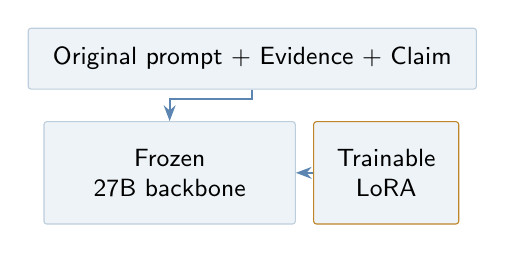
\begin{tikzpicture}
\node[box,text width=5.2cm] (input) at (0,1.3) {Original prompt + Evidence + Claim};
\node[box,text width=2.7cm,minimum height=1.3cm] (base) at (-1.05,-.15) {Frozen\\27B backbone};
\node[box,draw=Gold,text width=1.35cm,minimum height=1.3cm] (adapter) at (1.7,-.15) {Trainable\\LoRA};
\draw[flow] (input.south) -- ++(0,-.12) -| (base.north);
\draw[flow] (adapter.west)--(base.east);
\end{tikzpicture}
\end{center}
\small Seeds: 42, 43, 44\par
LoRA rank: 8\par
Update adapter parameters only
\end{column}
\begin{column}{.49\textwidth}
{\color{Blue}\textbf{Training data preparation}}\par
\smallbody
902 candidate items\par
$\downarrow$ AI-assisted item review\par
Remove 174 items by scenario group\par
$\downarrow$\par
\textbf{728 training items}
\vspace{.20cm}
\begin{beamercolorbox}[sep=.14cm,wd=\linewidth]{code}
\texttt{[Reviewed brief rationale]}\par
\texttt{Verdict: [Gold label]}
\end{beamercolorbox}
\end{column}
\end{columns}
\takeaway{Supervision changes model behavior while the prompt stays fixed.}
\source{Source: V16 revision 2 protocol and training-data review. Rationales were reviewed with AI assistance; they are not independent expert gold annotations. The supervision block is a format schematic.}
\note{LoRA changes trainable adapter parameters while keeping the backbone frozen and the original prompt fixed. We reviewed 902 candidate training items with AI assistance and removed 174 by whole scenario group, leaving 728. The targets combine a reviewed rationale with the correct label. Rank eight adapters were trained with three random seeds to measure variation. These rationales are not independent expert annotations.}
\end{frame}

% 09 -- 20 seconds
\begin{frame}[t]{Can Prompting and Fine-Tuning Work Together?}
\subtitleline{V18 explores three ways of combining the earlier routes.}
\vspace{.25cm}
\begin{tabularx}{\textwidth}{L{3.2cm}Y}
\rowcolor{Blue}\hc{Design}&\hc{Information flow}\\
\rowcolor{Pale}\textbf{Prompt\newline combination}&LoRA model + NLI / PJ prompt $\longrightarrow$ Final answer\\[.16cm]
\textbf{Disagreement\newline review}&Initial answers $\longrightarrow$ All valid and unanimous?\newline Yes: return answer. No: one review.\\[.16cm]
\rowcolor{Pale}\textbf{Rationale\newline distillation}&NLI / PJ / Joint rationales $\longrightarrow$ Item review\newline $\longrightarrow$ New LoRA $\longrightarrow$ One model call\\
\end{tabularx}
\vspace{.35cm}
\takeaway{Can the gains from prompting and fine-tuning accumulate?}
\source{Source: V18 experiment design. Rationales come from different prompting routes, not a larger teacher model. The completed quick scope and deferred full-scope components are reported separately.}
\note{We try three combinations: changing the prompt used with LoRA, reviewing disagreements among initial answers, and using reviewed explanations to train new adapters. The explanation sources are different prompts on the model, rather than a larger teacher.}
\end{frame}

% 10 -- 15 seconds
\begin{frame}[t]{A Unified Comparison Protocol}
\subtitleline{V17 compares every method on the same development items.}
\begin{columns}[T,onlytextwidth]
\begin{column}{.46\textwidth}
{\color{Blue}\textbf{Controlled conditions}}\par
\begin{itemize}
\item Same BF16 27B backbone
\item Thinking disabled; greedy decoding
\item Same rationale-and-verdict format
\item 1,024-token generation limit
\end{itemize}
\end{column}
\begin{column}{.49\textwidth}
\smallbody
\begin{tabularx}{\linewidth}{L{2.1cm}rY}
\rowcolor{Blue}\hc{Split}&\hc{N}&\hc{Use}\\
\rowcolor{Pale}Train&728&Learn parameters\\
Validation&259&Select checkpoints\\
\rowcolor{Pale}Development&261&Compare methods\\
\end{tabularx}
\vspace{.18cm}
\textbf{Comparison: 120 basic + 141 challenge}\par
Three seeds evaluated separately.\par
No voting or best-seed selection.
\end{column}
\end{columns}
\takeaway{Scenario groups are separated; this is historical development evidence.}
\source{Source: V17 comparison protocol and V16 revision 2 splits. Prior development exposure prevents an independent blind-test interpretation. Invalid outputs count as errors. The token number is a generation limit, not measured cost.}
\note{The unified comparison controls the backbone, decoding and output protocol. It evaluates 120 basic and 141 challenge items, with invalid outputs counted as errors. Scenario groups are separated for this run, but prior data exposure means these are development results, not a blind test.}
\end{frame}

% 11 -- 25 seconds
\begin{frame}[t]{LoRA Achieves the Highest Challenge Accuracy}
\subtitleline{Accuracy under the same V17 comparison protocol}
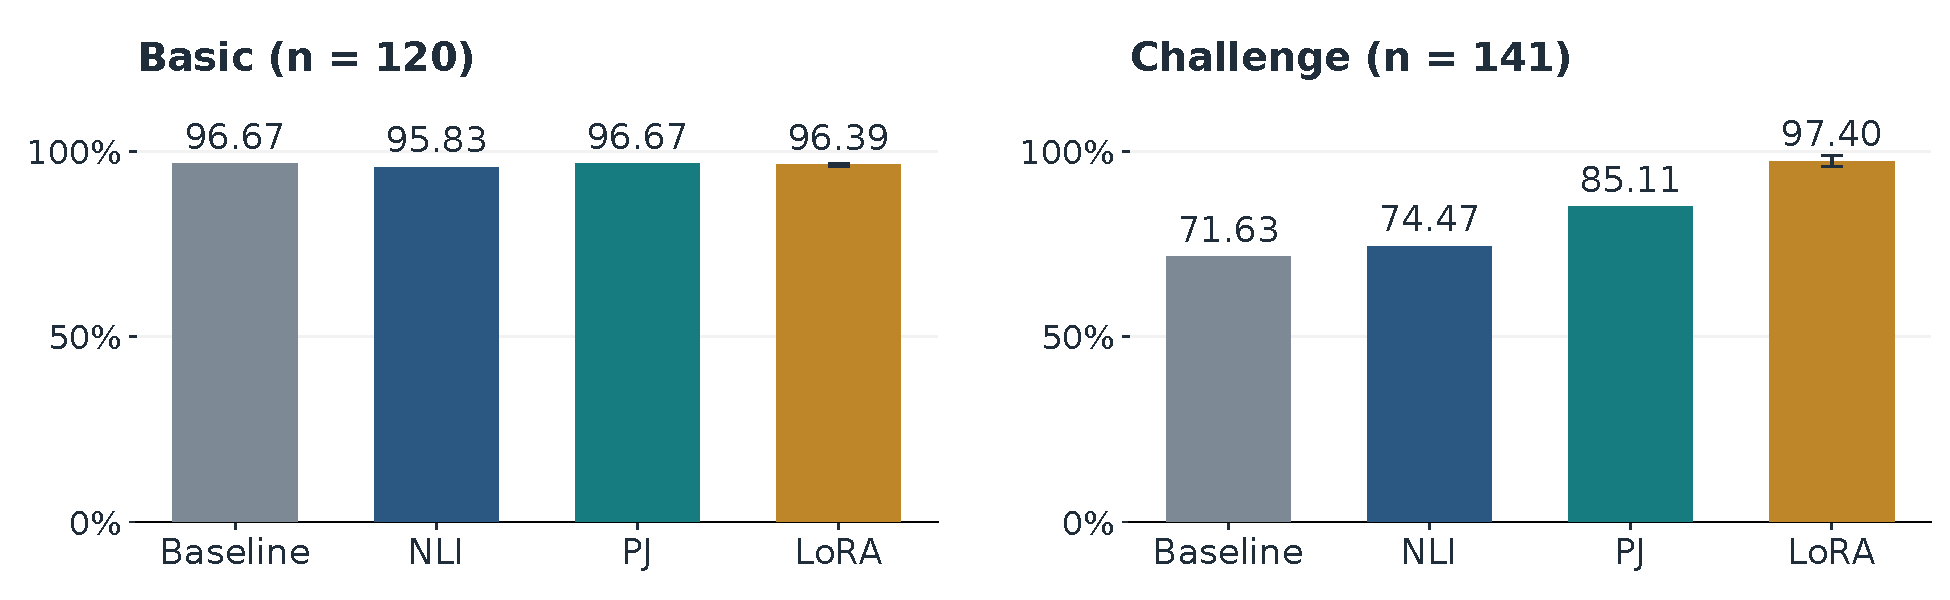
\includegraphics[width=\textwidth]{assets/accuracy.pdf}
\vspace{-.12cm}
\begin{columns}[T,onlytextwidth]
\begin{column}{.46\textwidth}
{\color{Teal}\textbf{PJ: +13.48 pp on challenge}}
\end{column}
\begin{column}{.50\textwidth}
{\color{Gold}\textbf{LoRA: +25.77 pp on challenge}}\par
\small Basic accuracy changes by $-0.28$ pp.
\end{column}
\end{columns}
\source{Source: V17 frozen results. LoRA: three-seed mean; error bars: sample SD (basic 0.48 pp, challenge 1.48 pp).\\Previously used development data, not an independent blind test. Invalid outputs count as errors.}
\note{The baseline reaches 71.63 percent on challenge items. NLI gives a modest gain, PJ reaches 85.11 percent, and LoRA averages 97.40 percent. Basic accuracy remains close to the baseline. The error bars show variation across three training seeds, not a generalization confidence interval.}
\end{frame}

% 12 -- 25 seconds
\begin{frame}[t]{Improvements on Difficult NEI Subtypes}
\subtitleline{Correct counts on the same selected items, before and after optimization}
{\fontsize{8.1}{10}\selectfont
\begin{tabularx}{\textwidth}{Yrrrr}
\rowcolor{Blue}\hc{NEI subtype}&\hc{Baseline}&\hc{NLI}&\hc{PJ}&\hc{LoRA range}\\
\rowcolor{Pale}A relative wins; claim concerns the subject&0/5&0/5&1/5&4--5/5\\
Pronoun refers to another person&0/3&0/3&2/3&\textbf{3/3}\\
\rowcolor{Pale}Another person succeeds; claim concerns the subject&0/2&1/2&1/2&2/2\\
A subset list is treated as complete&1/2&1/2&2/2&1--2/2\\
\rowcolor{Pale}An award this year; claim concerns an earlier year&0/3&0/3&2/3&1--3/3\\
Service after the first term&1/3&1/3&1/3&\textbf{3/3}\\
\rowcolor{Pale}Reports dismissed as baseless&0/4&1/4&\textbf{4/4}&\textbf{4/4}\\
\end{tabularx}}
\takeaway{Several zero-correct baseline subtypes improve.}
\small LoRA gains are broader, with some variation across seeds.
\source{Source: V17 predictions joined by item ID to V16 revision 2 development variants. Selected NEI subtypes only: 22 items. Post-hoc diagnosis, not an overall score or independent significance claim. Ranges show correct counts across three seeds.}
\note{The gains also appear in the difficult subtypes highlighted by Team A. Pronoun reference, first-term scope and baseless-report cases improve. These are selected NEI cases on our own comparison items: only 22 questions, used for post-hoc diagnosis. We do not compare Team A's local zero scores with our overall accuracy.}
\end{frame}

% 13 -- 20 seconds
\begin{frame}[t]{Where Do the Errors Go?}
\subtitleline{V17 challenge development set: 141 items. Each cell shows a percentage within its true class.}
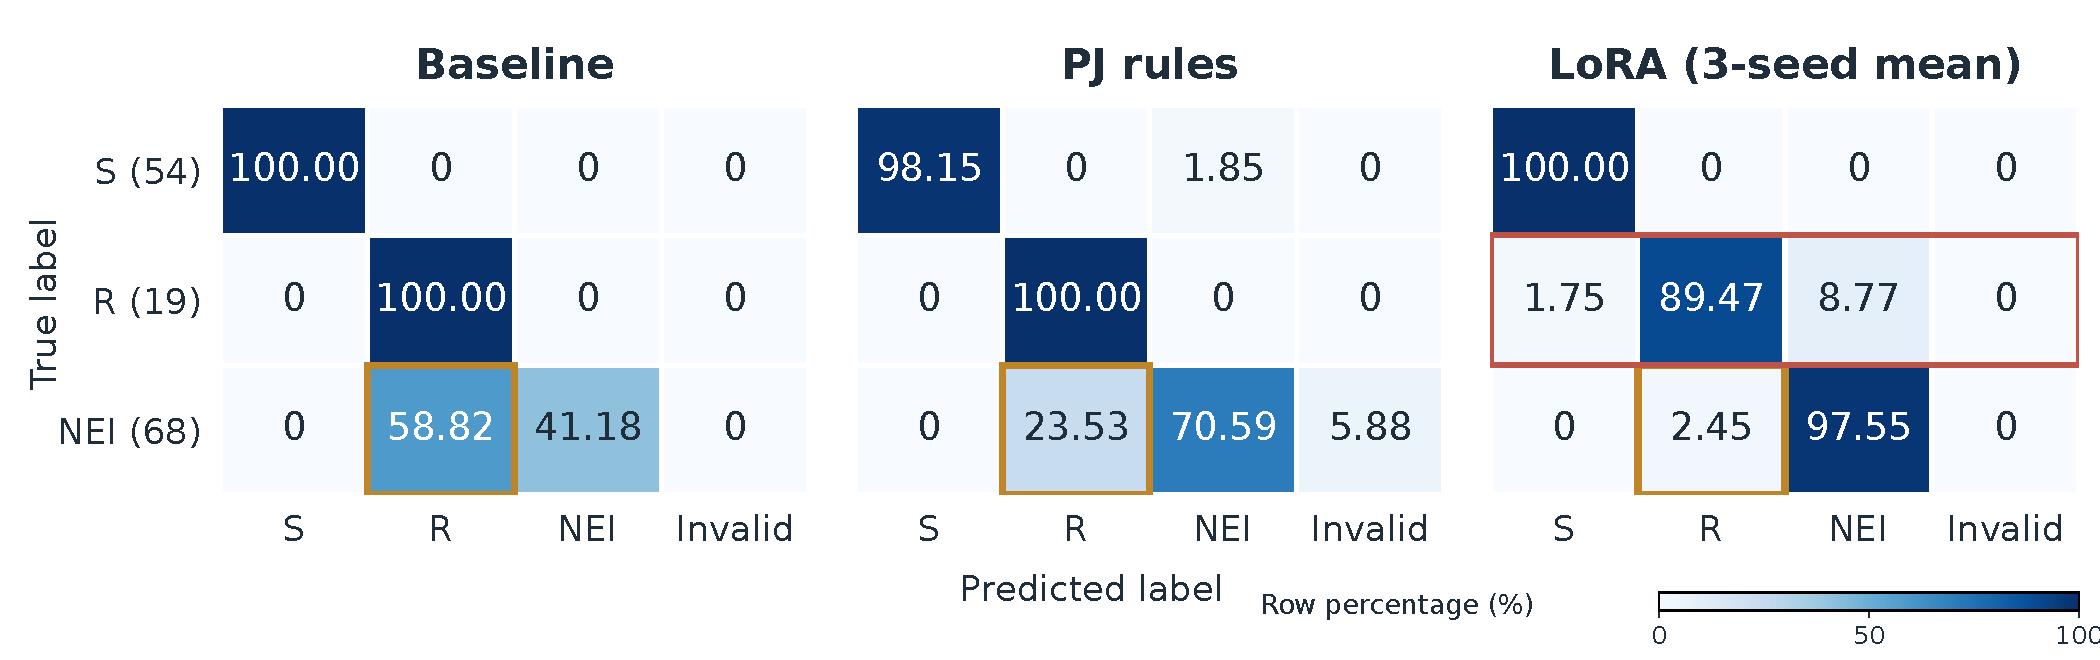
\includegraphics[width=\textwidth]{assets/confusion_main.pdf}
\vspace{-.17cm}
{\fontsize{7.6}{9.1}\selectfont S = SUPPORTS\quad R = REFUTES\quad NEI = NOT ENOUGH INFO\quad Invalid = invalid output}
\vspace{.14cm}
\begin{columns}[T,onlytextwidth]
\begin{column}{.52\textwidth}
{\color{Blue}\textbf{NEI $\rightarrow$ REFUTES}}\par
58.82\% $\rightarrow$ 23.53\% $\rightarrow$ 2.45\%
\end{column}
\begin{column}{.44\textwidth}
{\color{Red}\textbf{REFUTES recall}}\par
100\% $\rightarrow$ 100\% $\rightarrow$ 89.47\%
\end{column}
\end{columns}
\source{Source: V17 frozen predictions. LoRA averages row-normalized matrices from seeds 42, 43 and 44; no voting. Invalid outputs remain in the denominator. Frozen labels; historical development data. LoRA exceeds the 5 pp REFUTES regression limit; PJ alone meets all V17 criteria.}
\note{The baseline misclassifies 40 of 68 NEI items as REFUTES. PJ reduces this to 16; LoRA makes one, zero and four such errors across three seeds. However, every LoRA seed also misses two of the nineteen REFUTES items. This exceeds the preset regression limit.}
\end{frame}

% 14 -- 15 seconds
\begin{frame}[t]{Distillation Does Not Exceed Original LoRA}
\subtitleline{V18 quick scope: challenge accuracy on 141 development items}
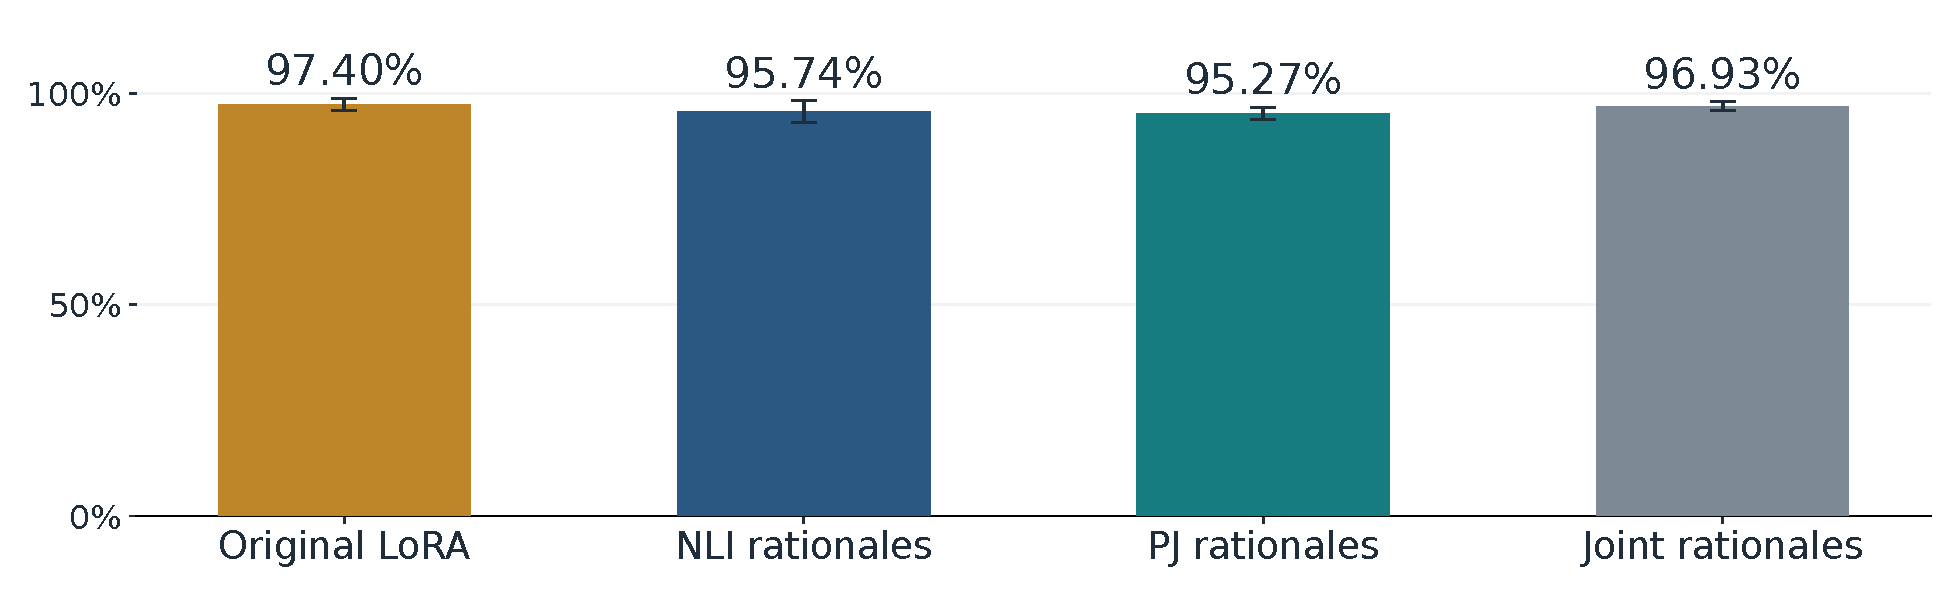
\includegraphics[width=\textwidth]{assets/distillation.pdf}
\vspace{-.14cm}
\small\textbf{Completed:} 9 training runs, 35 validation configurations, 13 development configurations.
\takeaway{No new distillation family meets all success criteria.}
\source{Source: V18 quick24 final assessment. Three-seed means with sample SD. Differences are not significant after multiple-comparison correction. New adapters use epoch 3; original LoRA retains prior checkpoint selection. Full-scope components remain deferred.}
\note{The completed distillation variants do not exceed original LoRA's mean challenge accuracy. None meets all success criteria. The differences are not statistically significant after correction, so we do not claim a significant decline. The full experiment still has deferred components.}
\end{frame}

% 15 -- 25 seconds
\begin{frame}[t]{What We Need to Validate Next}
\vspace{.14cm}
{\smallbody
\begin{tabularx}{\textwidth}{L{5.0cm}Y}
\rowcolor{Blue}\hc{Observed limitation}&\hc{Next step}\\
\rowcolor{Pale}Unclear rule contributions and coverage gaps&Add presupposition and time-scope rules; ablate rules individually\\[.13cm]
Higher NEI recall but lower REFUTES recall&Add explicit refutation / NEI contrasts; independently adjudicate disputed labels\\[.13cm]
\rowcolor{Pale}Prior data exposure and similar templates&Evaluate newly collected, unseen items; vary wording and compare inference cost\\
\end{tabularx}}
\vspace{.25cm}
\takeaway{Prompting and fine-tuning improve development results.}
\vspace{.05cm}
\textbf{Class trade-offs and generalization still need validation.}
\source{Planned work, not completed experiments. Current evidence uses historical development items and AI-assisted rationale review. Label disputes and data-sealing deviations are documented in the appendix.}
\note{Our next steps target the unresolved boundaries. We will isolate the effects of individual rules, add refutation and NEI contrasts, and independently resolve disputed labels. Most importantly, we need newly collected evaluation items and measured inference cost. Current gains are promising development evidence, with clear limits.}
\end{frame}

\appendix
% 16 -- backup
\begin{frame}[t]{Lessons from Earlier Attempts}
\subtitleline{Appendix: findings from separate experiment rounds}
{\fontsize{8.3}{10.4}\selectfont
\begin{tabularx}{\textwidth}{L{2.4cm}YY}
\rowcolor{Blue}\hc{Attempt}&\hc{Observation}&\hc{Lesson}\\
\rowcolor{Pale}Two-world reasoning&Counterexamples sometimes altered evidence or added exceptions&Preserve every evidence constraint\\
JSON constraints&V2: 441/441 formal outputs were valid JSON; semantic errors remained&Format validity does not guarantee correct reasoning\\
\rowcolor{Pale}Four-role construction and verification&V5 challenge: baseline 30/44; four-role method 18/44&Extra verification can introduce errors\\
Semantic formalization + Z3&V6: 42 valid JSON outputs, 24 executable ASTs; challenge 7/21 vs. baseline 14/21&Translation and representation were major bottlenecks\\
\end{tabularx}}
\takeaway{Faithful interpretation remains essential at every stage.}
\source{Sources: V2 RESULTS; V5 RESUMPTION\_20261026\_RESULTS; V6 RESULTS. Different subsets and protocols; these scores do not form a unified performance curve or establish that the methods fail in general.}
\end{frame}

% 17 -- backup
\begin{frame}[t]{Zero on a Subtype Is Not Zero Overall}
\subtitleline{Appendix: denominators explain apparently conflicting scores}
\vspace{.2cm}
\begin{columns}[T,onlytextwidth]
\begin{column}{.45\textwidth}
{\color{Blue}\large\textbf{AMBIGREF: V17 baseline}}\par
\vspace{.3cm}
SUPPORTS: \textbf{9/9} correct\par
NEI: \textbf{0/6} correct\par
\vspace{.26cm}
{\Large\color{Blue}Total: $9/15 = 60\%$}
\end{column}
\begin{column}{.49\textwidth}
{\color{Blue}\large\textbf{All challenge items}}\par
\vspace{.3cm}
Correct: 54 SUPPORTS\par
\hspace{1.4cm}+ 19 REFUTES + 28 NEI\par
\vspace{.26cm}
{\Large\color{Blue}$101/141 = 71.63\%$}
\end{column}
\end{columns}
\vspace{.50cm}
\takeaway{A subtype's 0\% does not imply 0\% on the whole mechanism.}
\source{Sources: V17 predictions and development variants; Team A reference deck. Team A reports 66.7\% overall challenge accuracy on slide 12. Its low-score denominators on slides 8--9 are not explicit. We reproduce related error patterns, not an exact recalculation of those percentages.}
\end{frame}

% 18 -- backup
\begin{frame}[t]{Difficult Subtypes: Results by Seed}
\subtitleline{Appendix: correct counts for the 22-item NEI diagnostic subset}
{\fontsize{7.5}{9.4}\selectfont
\setlength{\tabcolsep}{3.5pt}
\begin{tabularx}{\textwidth}{Yrrrrrrr}
\rowcolor{Blue}\hc{Mechanism / variant}&\hc{N}&\hc{Base}&\hc{NLI}&\hc{PJ}&\hc{L42}&\hc{L43}&\hc{L44}\\
\rowcolor{Pale}LOOKALIKE / bare&5&0&0&1&4&5&5\\
AMBIGREF / diff\_gender\_other\_pronoun&3&0&0&2&3&3&3\\
\rowcolor{Pale}UNIQUE / other\_indef\,|\,indef&2&0&1&1&2&2&2\\
SETCLOSE / subset\_count&2&1&1&2&2&2&1\\
\rowcolor{Pale}PRESUP / still\_decoy\,|\,before&3&0&0&2&3&3&1\\
TEMPSCOPE / first\_term&3&1&1&1&3&3&3\\
\rowcolor{Pale}DENIAL / baseless&4&0&1&4&4&4&4\\
\midrule\textbf{Total}&\textbf{22}&\textbf{2}&\textbf{4}&\textbf{13}&\textbf{21}&\textbf{22}&\textbf{19}\\
\end{tabularx}}
\vspace{.25cm}
\small Base = Baseline. L42 / L43 / L44 = LoRA seeds 42 / 43 / 44.
\source{Source: V17 predictions joined to V16 revision 2 development variants. Post-hoc selected NEI items only; variant fields are not model inputs. Seeds do not create extra independent items. PRESUP includes only the three NEI-labeled cases of the specified variant.}
\end{frame}

% 19 -- backup
\begin{frame}[t]{Limitations and Open Questions}
\subtitleline{Appendix: how to interpret the current results}
\begin{columns}[T,onlytextwidth]
\begin{column}{.43\textwidth}
{\color{Blue}\textbf{Evidence limits}}\par
\smallbody
\begin{itemize}
\item Prior development-data exposure
\item AI-assisted rationale review
\item No PRESUP training coverage
\item Some label interpretations remain disputed
\end{itemize}
\end{column}
\begin{column}{.53\textwidth}
\smallbody
{\color{Blue}\textbf{Which method is best?}}\par
LoRA has the highest V17 challenge accuracy. PJ alone meets all V17 criteria.
\vspace{.12cm}\par
{\color{Blue}\textbf{Why did fusion not improve further?}}\par
The completed designs did not meet all criteria. The cause has not been isolated.
\vspace{.12cm}\par
{\color{Blue}\textbf{What remains unfinished?}}\par
49 full-scope comparison configurations, added post-distillation review, epoch-wise selection and independent evaluation.
\end{column}
\end{columns}
\source{Sources: V16 revision 2 DEVIATIONS; V18 quick24 ASSESSMENT. V16 engineering tests read raw full/test files for overlap and deduplication checks. Those reads were not used for this run's model training, selection or evaluation, but strict data-sealing acceptance was not fully satisfied. V18's final five-family selection excluded standalone PJ.}
\note{V18 selected among five predefined method families that excluded standalone PJ prompting. Its fallback to A0 therefore does not invalidate the V17 comparison.}
\end{frame}

% 20 -- backup
\begin{frame}[t]{Confusion Matrices by Method and Seed}
\subtitleline{Appendix: cell text shows item counts; color shows the percentage within each true class.}
\begin{center}
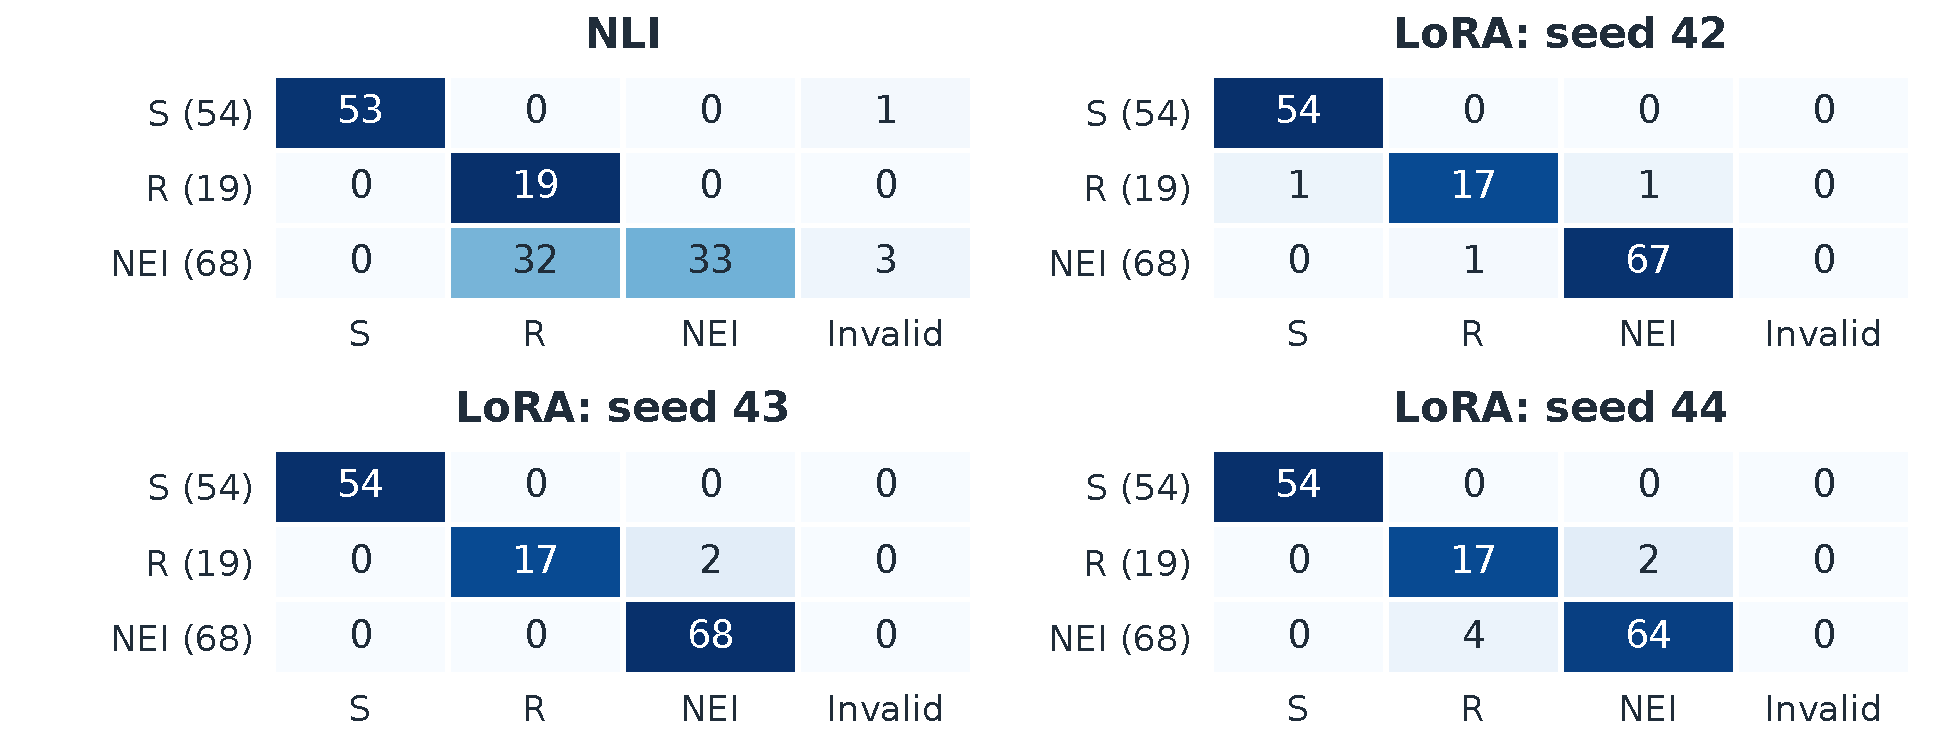
\includegraphics[width=.88\textwidth]{assets/confusion_seeds.pdf}
\end{center}
\vspace{-.2cm}
{\fontsize{7.4}{9}\selectfont Rows: true label. Columns: predicted label. S = SUPPORTS; R = REFUTES; NEI = NOT ENOUGH INFO.}
\source{Source: V17 frozen predictions. Every panel uses the same 141 challenge items; row counts are 54, 19 and 68. Shared color scale: 0--100\%. Invalid outputs count as errors. Each seed is a separate run, not an extra independent set of items.}
\end{frame}

\end{document}
